\documentclass[11pt]{beamer}

\usepackage[T1]{fontenc}
\usepackage[utf8x]{inputenc}
\usepackage{natbib}

%% Fonts
\usepackage{multicol}
\usepackage{mathabx}
\usepackage[scaled]{helvet}
\usepackage{lmodern}
\usepackage{eulervm}
\usefonttheme[onlymath]{serif}
\usefonttheme{professionalfonts}
\usefonttheme{structurebold}

\usepackage{hyperref}

\usepackage{bm}
\usepackage{pgf}
\usepackage{natbib}


\DeclareMathOperator*{\argmax}{arg\,max}


%% Color & Theme
\usetheme{AnnArbor}

\setbeamerfont{title}{size=\large}
\setbeamerfont{frametitle}{size=\large}

\definecolor{SUblue}{RGB}{0,0,180}
% \usecolortheme[RGB={0,0,180}]{structure}
% \usetheme{Boadilla}
\setbeamertemplate{navigation symbols}{}
% \setbeamertemplate{itemize items}[circle]
% \setbeamertemplate{enumerate items}[circle]
% \setbeamerfont{title}{size=\large}
% \setbeamerfont{frametitle}{size=\large}
\setbeamerfont{framesubtitle}{size=\large,shape =$\color{violet}{\looparrowdownright}~$}
% \setbeamercolor{title}{fg=white, bg= SUblue!75!green}
% \setbeamercolor{framesubtitle}{fg=violet}
% \setlength{\leftmargini}{5pt}


% \hypersetup{colorlinks=true, linkcolor=blue}

\title[Bayesian Response Surface Maximization]{Efficient Bayesian Response Surface Maximization}


\author[Feng
Li]{\includegraphics[height=2cm]{cufelogo}\\\vspace{0.5cm}\textbf{Feng
    Li}}

\institute[Stat\&Math, CUFE]{\footnotesize{\textbf{School of
      Statistics and Mathematics\\ Central University of Finance and
      Economics}\\ \texttt{Email: feng.li@cufe.edu.cn}}}

\date{}


%%%%%%%%%%%%%%%%%%%%%%%%%%%%%%%%%%%%%%%%%%%%%%%%%%%%%%%%%%%%%%%%%%%%%%%%%%%%%%%
\begin{document}


%% Title page
\begin{frame}[plain]
  \titlepage
  % \tiny{Revision: \today}
\end{frame}

%% Outline page
\section*{Outline}
\begin{frame}
  \frametitle{Outline}
  \tableofcontents
\end{frame}

\section{Introduction: An Economics Data Example}
\begin{frame}
  \frametitle{The firm leverage data}
  \vspace{0.25cm}
  \scalebox{0.60}{
    \begin{tabular}{rl}
      \textbf{leverage ($Y$):} &total debt/(total debt+book value of equity), 4405 observations;\\
      \textbf{tang:} & tangible assets/book value of total assets;\\
      \textbf{market2book:} &(book value of total assets - book value of equity +
      market value of equity) / book value of total assets;\\
      \textbf{logSales:} &logarithm of sales;\\
      \textbf{profit:} &(earnings before interest, taxes, depreciation, and amortization) /
      book value of total assets.    \\
    \end{tabular}}
  \vspace{0.25cm}
  \begin{center}
    \begin{figure}
      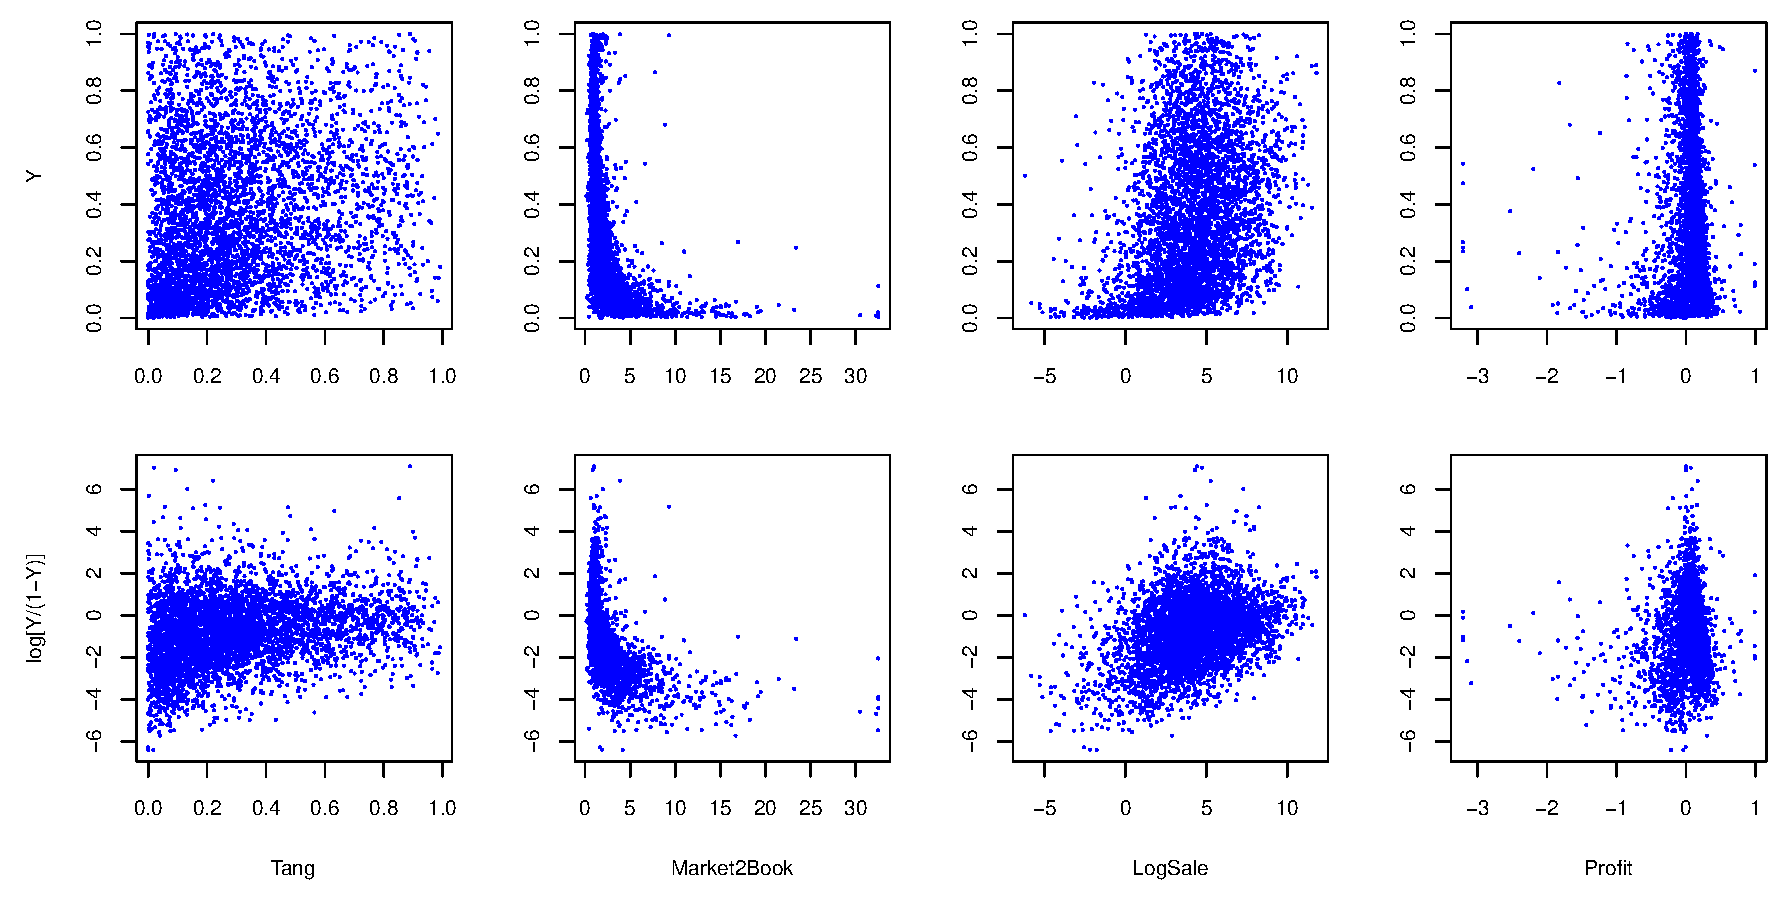
\includegraphics[width=\textwidth]{Rajanscatter.eps}
    \end{figure}
  \end{center}

\end{frame}

\begin{frame}
  \frametitle{Our interests}

  \begin{itemize}
  \item Find an optimal combination of \textbf{tang},
    \textbf{market2book}, \textbf{logSales}, and \textbf{profis} so
    that \textbf{leverage} reaches the maximum.

  \item We may write it down in mathematics

    \begin{equation*}
      \argmax_{\bm{x} \in R^d} ~ f(\bm{x})
    \end{equation*}
    where $ \bm{x}$ is defined as sample and $\bm{y} = f (\bm{x}) +
    \bm{\epsilon} $ with $\bm{\epsilon}$ as the noisy observation of
    the objective function at $\bm{x}$.

  \item But note that

    \begin{itemize}
    \item The function $f(\bm{x})$ is \textbf{unknown}, \textbf{not
        noise-free} and \textbf{hard to evaluate}.
    \item We do not know its derivatives. Common optimization methods
      usually fail here.
    \item The covariates space can be very sparse.
    \end{itemize}

  \end{itemize}

\end{frame}

\section{Bayesian Response Surface Maximization}

\begin{frame}[allowframebreaks]
  \frametitle{Bayesian Optimization}

  \begin{enumerate}
  \item Assume $D_{1:t} = {\bm{x}_{1:t} , \bm{y}_{1:t} }$ are
    observations, a prior distribution $P (f )$ over function $f(\cdot)$ is
    combined with the likelihood function $P (D_{1:t} |f )$ to produce
    the posterior distribution

    \begin{equation*}
      P (f|D_{1:t} ) \propto P (D_{1:t} |f )P (f ).
    \end{equation*}

  \item Bayesian optimization it to find $\bm{x}_{t+1}$
    \begin{equation}
      \label{eq:bayes-optim}
      \bm{x}_{t+1} = \argmax_{\bm{x} \in R^d} \int a(\bm{x})  P (f_{t+1}|D_{1:t}
      )d f_{t+1}
    \end{equation}
    where $a(x)$ is called \textbf{acquisition function}
    that guides the search for the optimum that high acquisition
    corresponds to potentially high values of the objective function.

  \end{enumerate}
  \begin{itemize}
  \item Common acquisition functions include \textbf{probability of
      improvement}, \textbf{expected improvement} and \textbf{entropy}
    \citep{kushner1964new, mockus1978application,jones2001taxonomy,
      cox1997sdo,brochu2010hedging, villemonteix2009informational}

  \item Recent work in Bayesian Optimization like
    \citet{jones1998efficient} \citet{jones2001taxonomy},
    \citet{bergstra2012random} can trace back to
    \citet{cox1997sdo}.

  \item Bayesian Optimization is a popular approach in engineering but
    not well known in statistics.

    \newpage
  \item We are interested in finding the maximum for the predictive surface

    \[p(\tilde{y}_{b}|\tilde{y}_{-b},x)=\int\prod_{i\in\mathcal{T}_{b}}p(y_{i}|\theta,x_{i})p(\theta|\tilde{y}_{-b})\mathrm{d}\theta,\]

  \item However in econometric time series this is much more
    complicated due to the decomposition

    \begin{align*}
      % \label{eq:predict}
      &p(Y_{(T+1):(T+p)}|Y_{1:T},X)\\
      &=\prod\limits _{i=1}^{p}\int
      p(Y_{T+i}|\theta,Y_{1:(T+i-1)}, X_{T+i})p(\theta|Y_{1:(T+i-1)},X_{{1:(T+i-1)}})\mathrm{d}\theta.
    \end{align*}

  \end{itemize}
\end{frame}

\begin{frame}[allowframebreaks]
  \frametitle{Bayesian modeling of $P (f|D_{1:t} )$}
  \begin{itemize}
  \item The function $f(x)$ is usually approximated by a Gaussian
    Process \citep{mockus1994application, sasena2002flexibility}
    \begin{equation*}
      f(\bm{x})=\mathcal{GP}(m(\bm{x}),k(\bm{x},\bm{x}'))
    \end{equation*}
    which is restrictive by $\mathcal{GP}$ itself because choosing the
    covariance function for the $\mathcal{GP}$ is crucial.

  \item We consider the \textbf{multivariate surface model}
    \citep{li2013efficient} to model $f(x)$

    \begin{itemize}
    \item The surface consists of three different components,
      {\color{blue}\emph{linear}}, {\color{blue}\emph{surface}} and
      {\color{blue}\emph{additive}} as
      \[\begin{gathered}
        \bm{Y}=\bm{X}_o\bm{B}_o+
        \bm{X}_s(\xi_s)\bm{B}_s+\bm{X}_a(\xi_a)\bm{B}_a + \bm{E}.
      \end{gathered}\]
    \item We treat the knots $\xi_i$ as unknown parameters and let them move
      freely.
    \item A model with a minimal number of free knots outperforms model with lots
      of fixed knots.
    \item For notational convenience, we sometimes write model in compact form
      \[
      \bm{Y}=\bm{X}\bm{B}+\bm{E},
      \]
      where $\bm{X}=[\bm{X}_{o},\bm{X}_{s},\bm{X}_{a}]$ and
      $\bm{B}=[{\bm{B}_{o}}',{\bm{B}_{s}}',{\bm{B}_{a}}']'$ and $\bm{E}\sim \bm{N}_p(\bm{0},~\bm{\Sigma})$
    \end{itemize}

  \end{itemize}

\end{frame}

\section{The Efficient MCMC algorithm}
\begin{frame}[allowframebreaks]
  \frametitle{The Efficient MCMC algorithm}
  \begin{itemize}
  \item The coefficients ($\bm{B}$) are directly sampled from normal distribution.
  \item We update covariance ($\bm{\Sigma}$), all knots ($\bm{\xi}$) and shrinkages ($\bm{\lambda}$) jointly by using
    Metropolis-Hastings within Gibbs.
  \item  The proposal density for $\bm{\Sigma}$ is the inverse Wishart
    density on previous slide.
  \item The proposal density for $\bm{\xi}$ and $\bm{\lambda}$ is a multivariate \emph{t}-density with $\nu>2$ df,
    \[
    \bm{\theta}_{p}|\bm{\theta}_{c}\sim\bm{MVT}\left[\bm{\hat{\theta}},~\left.-\left(\frac{\partial^{2}\ln
            p(\bm{\theta}|\bm{Y})}{\partial\bm{\theta}\partial\bm{\theta}^{\prime}}\right)^{-1}\right\vert
      _{\bm{\theta}=\bm{\hat{\theta}}},~\nu\right],
    \]
    where $\bm{\hat{\theta}}$ is obtained by $R$ steps ($R\leq 3$) Newton's
    iterations during the proposal with analytical gradients for matrices.

  \item The Metropolis-Hastings acceptance probability is
    \[
    a\left(\bm{\theta}_{c}\rightarrow\bm{\theta}_{p}\right)=\min\left[1,~\frac{p(\bm{Y}|\bm{\theta}_{p})p(\bm{\theta}_{p})g(\bm{\theta}_{c}|\bm{\theta}_{p})}{p(\bm{Y}|\bm{\theta}_{c})p(\bm{\theta}_{c})g(\bm{\theta}_{p}|\bm{\theta}_{c})}\right].
    \]

  \item The analytical gradients are very complicated and we have
    implemented it in an efficient way.

  \item Bayesian variable selection can be naturally applied in MCMC procedure.

  \item The MCMC implementations are straightforward.

  \item We allow the parameters to be updated via:
    \begin{itemize}
    \item parallel mode for small datasets,
    \item batched mode for big datasets.
    \end{itemize}


  \item MCMC method allows us to evaluate the integral in
    Eq. (\ref{eq:bayes-optim}) easily.

  \end{itemize}

\end{frame}


\begin{frame}
  \frametitle{Optimizing the acquisition function}

  \begin{itemize}
  \item With the posterior, a deterministic, derivative-free optimizer
    can then be used in optimizing the acquisition function
    \citep{jones1993lipschitzian, mockus1994application,
      lizotte2008practical}.

  \item By taking the advantage of MCMC, we may integrate the two steps
    together. \emph{Working in progress}...

  \end{itemize}

\end{frame}

\section{The firm leverage data, a revisit}

\begin{frame}
  \frametitle{The firm leverage data, a revisit}

  \begin{figure}
    \centering
    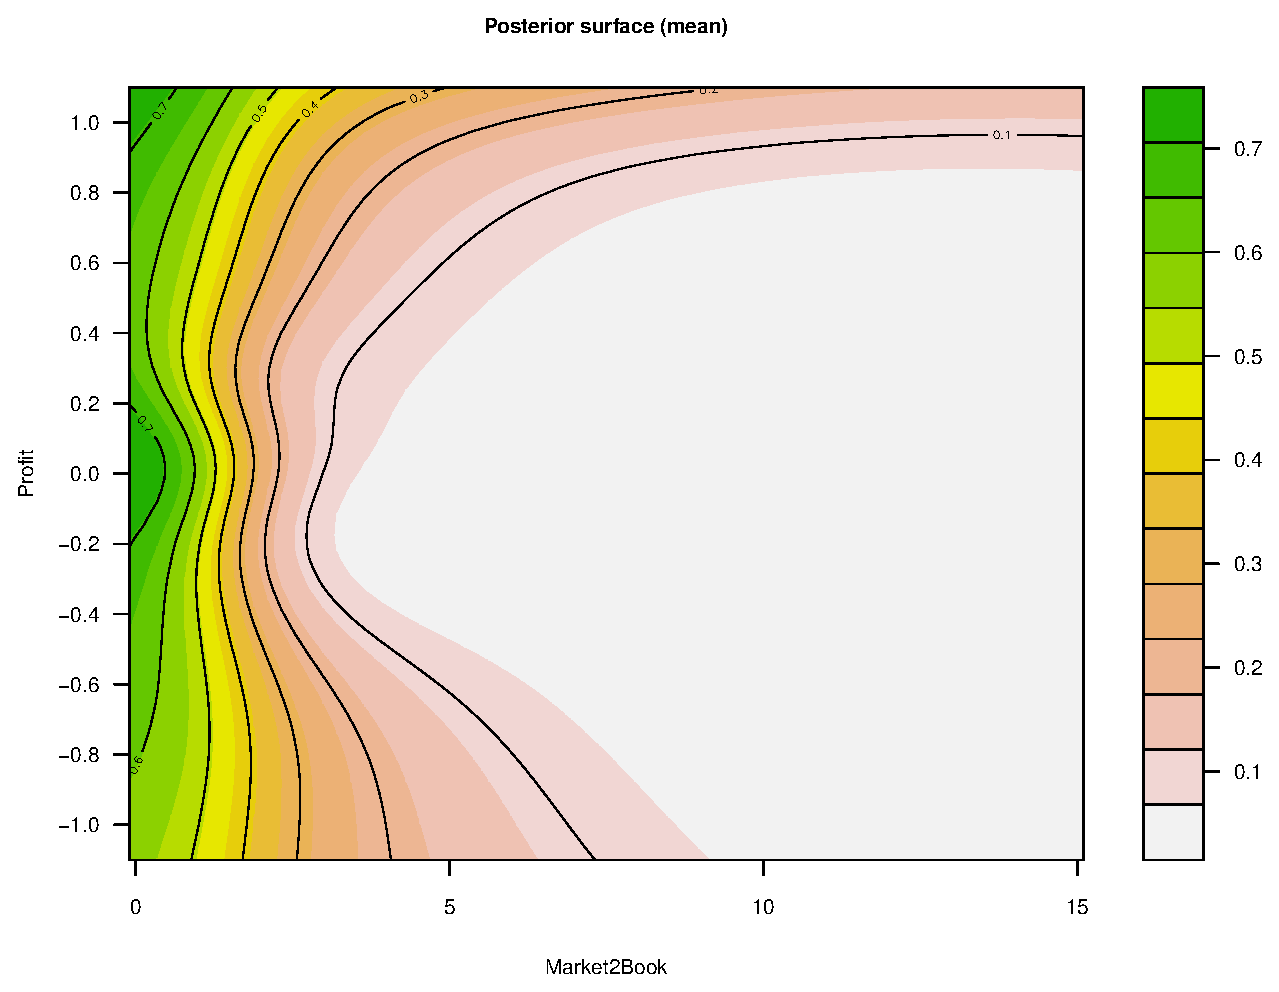
\includegraphics[trim= 0 0 0 0, height=0.85\textheight]{RajanPostMean}
  \end{figure}
\end{frame}


\begin{frame}
  \frametitle{Extensions}
  \begin{itemize}
  \item Our approach can be applied experimental design.
  \item High dimensional response surfaces will be considered.
  \end{itemize}
\end{frame}

\begin{frame}[allowframebreaks]
  \frametitle{References}
  \bibliography{References,full}
  \bibliographystyle{asa}
\end{frame}


\begin{frame}[plain]

  \addtocounter{framenumber}{-1}

  % \emph{...essentially, all models are wrong, but some are useful}\\
  % \hfill --- George E. P. Box
  \vspace{1cm}
  \begin{center}
    {\color{SUblue} \textbf{\Huge Thank you!}}
  \end{center}


\end{frame}
\end{document}
